Neironu tīklu agrīnā teorija aizsākās ap 1943. gadu, kad Vorens Makaloks un Volters Pitss \cite{mcculloch1943}
aprakstīja vienkāršotu bioloģiskā neirona matemātisko modeli. Šajā modelī neirons tika modelēts kā skaitļošanas vienība, kas
integrē svērtas ieejas un, izmantojot sliekšņa funkciju, rada bināru izeju. Šis darbs vēlāk lika pamatus vienam no
agrīnākajiem mācīšanās algoritmiem perceptronam, kas darbojas kā lineārs binārs klasifikators.

Neraugoties uz tā nozīmi, perceptrons bija piemērojams tikai lineāri atdalāmiem vektoriem, kas kavēja neironu tīklu
pētniecības sākotnējo attīstību. Šo periodu bieži dēvē par „mākslīgā intelekta ziemu” \cite{toosi2021}. Galu galā mūsdienu
dziļās mācīšanās attīstība \Gls{ann} jomā, piemēram, dziļas daudzslāņu arhitektūras un nelineāras aktivācijas funkcijas, ļāva
pārvarēt šos ierobežojumus.

Lai gan jaunākie sasniegumi uz \Gls{ann} balstītos dziļās mācīšanās modeļos ir devuši ievērojamus panākumus dažādos
lietojumos, tiem joprojām ir ierobežojumi, tostarp liels enerģijas patēriņš un lielas atmiņas prasības. Pieaugot modeļu
apjomam, ievērojami palielinās resursu prasības apmācības un plašas ieviešanas laikā, tādēļ arvien lielāka uzmanība tiek
pievērsta energoefektīvam mākslīgajam intelektam. Intelektuālo sistēmu arvien plašāka ieviešana perifērijas ierīcēs,
piemēram, autonomajos transportlīdzekļos un iegultajās platformās, vēl vairāk pastiprina vajadzību pēc energoefektīvas
skaitļošanas. Šādos gadījumos jaudas patēriņš un skaitļošanas resursi kļūst par kritiskiem ierobežojumiem, kas ierobežo
tradicionālo risinājumu mērogojamību \cite{lin2018}. Turklāt, lai gan tradicionālie \Gls{ann} spēj apstrādāt temporālu un uz
notikumiem balstītu informāciju, to tipiskās realizācijas balstās uz blīvām tenzoru operācijām fon Neimana arhitektūrās, kas
neizmanto asinhrono sensoru notikumu retuma priekšrocības. Jaunie retinomorfie sensori, piemēram, \Gls{dvs}
\cite{delbruck2008}, ir nodrošinājuši jauna veida notikumu datus ar augstu laika izšķirtspēju un retumu. Šie sensori rada
asinhronus notikumus blīvu attēlu kadru vietā, tādēļ tie nav saderīgi ar tradicionālo skaitļošanu.

Šie ierobežojumi ir veicinājuši interesi par alternatīvām skaitļošanas paradigmām, kuru iedvesmas avots ir bioloģiskās
neironu sistēmas. \Gls{snn} informāciju attēlo ar diskrētiem impulsu notikumiem laikrindās, nodrošinot retus un uz
notikumiem balstītus aprēķinus. Kā piedāvāts \cite{maass1997}, tie nodrošina bioloģiski reālistiskāku neirālās
apstrādes modeli un ir daudzsološs risinājums energoefektīvām neiromorfās skaitļošanas sistēmām. Turklāt sensori, kas rada
asinhronus notikumus, ir tieši saderīgi ar \Gls{snn} uz notikumiem balstīto apstrādi.

Neironu tīklus bieži iedala trijās paaudzēs \cite{maass1997}. Pirmā paaudze ietver vienkāršus sliekšņa modeļus, piemēram,
perceptronu. Pašlaik plaši izplatītā otrā paaudze ietver nepārtrauktas aktivācijas funkcijas, ko izmanto mūsdienu \Gls{ann},
piemēram, sigmoīdu un \Gls{relu}. Trešā paaudze, proti, \Gls{snn}, izmanto temporālo dinamiku, bioloģiski iedvesmotus neironu
modeļus un saziņu ar diskrētiem impulsiem.

Lai gan pašreizējie pētījumi demonstrē arvien plašāku \Gls{snn} algoritmisko piemērojamību ārpus tradicionālajiem uztveres
uzdevumiem, to energoefektivitātes priekšrocības joprojām ir atkarīgas no skaitļošanas aparatūras arhitektūras. Šo
priekšrocību īstenošanai nepieciešamas aparatūras arhitektūras, kas spēj izmantot uz notikumiem balstītus aprēķinus. Tādēļ
skaitļošanas aparatūras izvēlei ir būtiska nozīme \Gls{snn} realizāciju praktiskās efektivitātes noteikšanā.

\ref{fig:hw_tradeoff}. attēlā parādīts kompromiss starp skaitļošanas elastību un energoefektivitāti dažādās skaitļošanas
platformās. Lai gan CPU un GPU sistēmas nodrošina plašas programmēšanas iespējas un atbalsta dažādas neironu tīklu
arhitektūras, to energoefektivitāte ir ierobežota, jo tās nevar pilnībā izmantot uz notikumiem balstītu aprēķinu retumu.
Savukārt specializētas neiromorfās platformas balstītas uz \Gls{asic} sasniedz ievērojami augstāku efektivitāti, pateicoties
pielāgotai notikumu apstrādei, taču ar ļoti ierobežotu elastību. \Gls{fpga} sistēmas ir vidusceļš. Tās piedāvā
aparatūras pārkonfigurējamību un iespēju realizēt pielāgotas, uz notikumiem balstītas apstrādes un atmiņas arhitektūras,
vienlaikus izmantojot retu operāciju energoefektivitātes priekšrocības.

Tas motivē pētīt uz \Gls{fpga} balstītus impulsu neironu tīklu paātrinātājus, kas apvieno programmējamas aparatūras elastību
ar neiromorfās skaitļošanas efektivitāti.

\begin{figure}[h!]
\centering
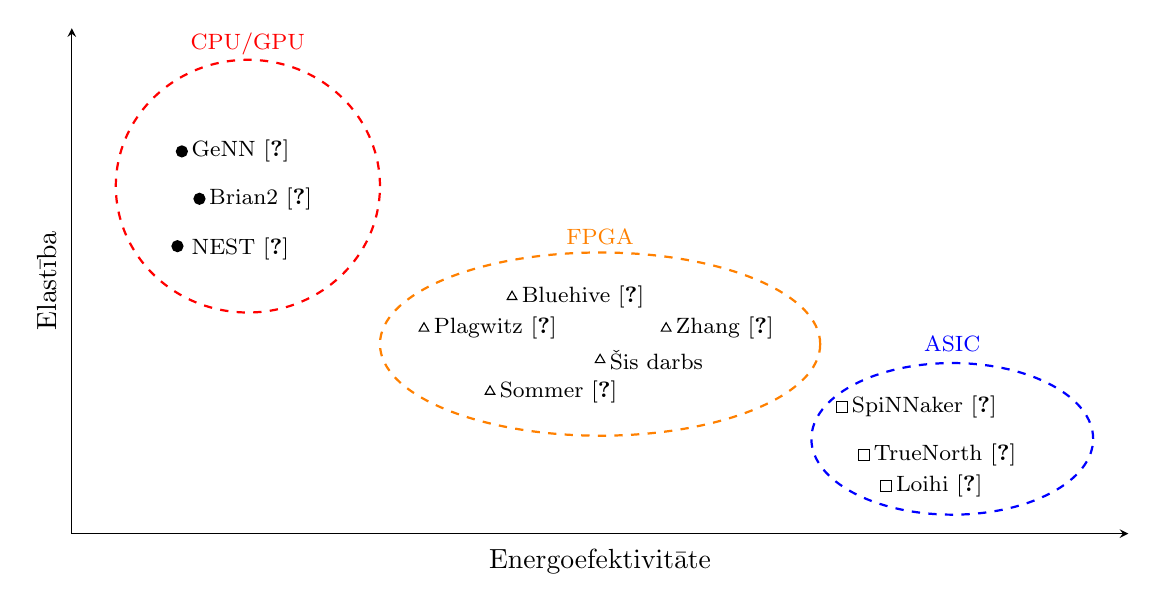
\begin{tikzpicture}
\def\Cx{4.0}
\def\Cy{11.0}
\def\Fx{12.0}
\def\Fy{6.0}
\def\Ax{20.0}
\def\Ay{3.0}
\begin{axis}[
    xlabel={Energoefektivitāte},
    ylabel={Elastība},
    xmin=0, xmax=24,
    ymin=0, ymax=16,
    xtick=\empty,
    ytick=\empty,
    axis lines=left,
    width=15cm,
    height=8cm
]

\addplot[only marks, mark=*] coordinates {(2.4,9.1)};
\node[anchor=west] at (axis cs:2.5,9.0) {\footnotesize NEST \cite{gewaltig2007}};

\addplot[only marks, mark=*] coordinates {(2.9,10.6)};
\node[anchor=west] at (axis cs:2.9,10.6) {\footnotesize Brian2 \cite{stimberg2019}};

\addplot[only marks, mark=*] coordinates {(2.5,12.1)};
    \node[anchor=west] at (axis cs:2.5,12.1) {\footnotesize GeNN \cite{yavuz2016}};

\addplot[only marks, mark=triangle] coordinates {(\Fx-2.5,\Fy-1.5)};
\node[anchor=west] at (axis cs:\Fx-2.5,\Fy-1.5) {\footnotesize Sommer \cite{sommer2022}};

\addplot[only marks, mark=triangle] coordinates {(\Fx-4.0,\Fy+0.5)};
\node[anchor=west] at (axis cs:\Fx-4.0,\Fy+0.5) {\footnotesize Plagwitz \cite{plagwitz2025}};

\addplot[only marks, mark=triangle] coordinates {(\Fx-2.0,\Fy+1.5)};
\node[anchor=west] at (axis cs:\Fx-2.0,\Fy+1.5) {\footnotesize Bluehive \cite{moore2012}};

\addplot[only marks, mark=triangle] coordinates {(\Fx+1.5,\Fy+0.5)};
\node[anchor=west] at (axis cs:\Fx+1.5,\Fy+0.5) {\footnotesize Zhang \cite{zhang2024}};

\addplot[only marks, mark=triangle] coordinates {(\Fx,\Fy-0.5)};
\node[anchor=west] at (axis cs:\Fx,\Fy-0.5) {\footnotesize Šis darbs};

\addplot[only marks, mark=square] coordinates {(\Ax-2.5,\Ay+1.0)};
\node[anchor=west] at (axis cs:\Ax-2.5,\Ay+1.0) {\footnotesize SpiNNaker \cite{furber2014}};

\addplot[only marks, mark=square] coordinates {(\Ax-2.0,\Ay-0.5)};
\node[anchor=west] at (axis cs:\Ax-2.0,\Ay-0.5) {\footnotesize TrueNorth \cite{akopyan2015}};

\addplot[only marks, mark=square] coordinates {(\Ax-1.5,\Ay-1.5)};
\node[anchor=west] at (axis cs:\Ax-1.5,\Ay-1.5) {\footnotesize Loihi \cite{orchard2021}};

\draw[blue, dashed, thick]
    (axis cs:\Ax,\Ay) ellipse (3.2 and 2.4);

\node[blue] at (axis cs:\Ax,6.0) {\footnotesize ASIC};

\draw[orange, dashed, thick]
    (axis cs:\Fx,\Fy) ellipse (5.0 and 2.9);

\node[orange] at (axis cs:\Fx,\Fy+3.4) {\footnotesize FPGA};

\draw[red, dashed, thick]
    (axis cs:\Cx,\Cy) ellipse (3.0 and 4.0);

\node[red] at (axis cs:\Cx,\Cy+4.5) {\footnotesize CPU/GPU};

\end{axis}
\end{tikzpicture}
\caption{Kompromiss starp energoefektivitāti un elastību dažādās SNN simulācijas un aparatūras platformās.}
\label{fig:hw_tradeoff}
\end{figure}

Šī pētījuma vispārējais mērķis ir izstrādāt un novērtēt pārkonfigurējamas, uz \Gls{fpga} balstītas impulsu neironu tīklu
paātrināšanas metodes, kas nodrošina mazas jaudas un zema latentuma inferenci attēlu klasifikācijai un objektu detektēšanai,
vienlaikus risinot dziļo impulsu neironu tīklu atmiņas mērogojamības ierobežojumus.

Šī mērķa sasniegšanai izvirzīti šādi pētnieciskie uzdevumi:
\begin{enumerate}
\item Izpētīt konvolucionālo impulsu neironu tīklu realizāciju aparatūrā un tās ierobežojumus, piemēram, svaru
  kvantēšanas ietekmi uz klasifikācijas veiktspēju, un noteikt \Gls{fpga} realizācijai piemērotu arhitektūru un skaitlisko
    precizitāti.

\item Izstrādāt un realizēt pārkonfigurējamu \Gls{fpga} paātrinātāju konvolucionālajiem impulsu neironu tīkliem, kas atbalsta
  dažādas tīklu konfigurācijas un impulsu neironu modeļus.

\item Izstrādāt un novērtēt atmiņas arhitektūru dziļāku tīklu atbalstam, apvienojot svaru glabāšanu mikroshēmā ar membrānas
  potenciālu straumēšanu ārpus mikroshēmas, lai samazinātu mikroshēmas iekšējās atmiņas prasības.

\item Izpētīt impulsu neironu tīklu piemērotību 3D objektu detektēšanai, izmantojot LiDAR un lidojuma laika punktu mākoņu
  reprezentācijas, tostarp novērtēt detektēšanas veiktspēju ar dažādām sensoru modalitātēm un iespējamās energoefektivitātes
    priekšrocības.

\item Eksperimentāli novērtēt \Gls{fpga} inferences latentumu, aparatūras resursu izmantojumu un jaudas patēriņu, kā arī
  izvērtēt piedāvāto impulsu neironu tīklu modeļu energoefektivitāti salīdzinājumā ar tradicionālajiem mākslīgajiem neironu
    tīkliem.

\end{enumerate}

Pētījuma mērķa un uzdevumu izpilde tiek novērtēta ar šādām trim tēzēm, kas attiecas uz aparatūras paātrināšanu un \Gls{snn}
arhitektūrāmu telpiski temporālu datu apstrādei:
\begin{itemize}

\item \textbf{1. tēze:} Impulsu neironu tīkls, kas realizēts pārkonfigurējamā \Gls{fpga} paātrinātājā un izmanto kvantētus
  svarus ar mazu bitu skaitu, saglabā klasifikācijas veiktspējas atšķirību 5~\% robežās no ekvivalenta pilnas precizitātes
    \Gls{snn} modeļa \textit{MNIST} un \textit{Caltech-101} veiktspējas testos, vienlaikus nodrošinot izmērīto dinamisko jaudas
    patēriņu zem 0,5~W un saglabājot elastību dažādām tīklu konfigurācijām un impulsu neironu modeļiem.

\item \textbf{2. tēze:} \Gls{snn} ir piemērojami 3D objektu detektēšanas uzdevumiem punktu mākoņu reprezentācijās, sasniedzot
  vismaz 70~\% vidējo precizitāti autonomās braukšanas transportlīdzekļu detektēšanas veiktspējas testā un vienlaikus nodrošinot
    analītiski novērtētu inferences enerģijas samazinājumu vismaz par 25~\% salīdzinājumā ar ekvivalentiem 3D objektu
    detektēšanas \Gls{ann} modeļiem.

\item \textbf{3. tēze:} Pārkonfigurējama konveijerizēta \Gls{fpga} arhitektūra, kas apvieno svaru glabāšanu mikroshēmā ar
  membrānas potenciālu straumēšanu ārpus tās, samazina iekšējās atmiņas prasības vismaz par 50~\%
    neiromorfajā \textit{Caltech-101} attēlu klasifikācijas veiktspējas testā, vienlaikus saglabājot inferences latentumu zem
    10~ms.

\end{itemize}

Šī promocijas darba galvenais ieguldījums ir divi savstarpēji papildinoši risinājumi: pārkonfigurējama, uz \Gls{fpga}
balstīta \Gls{snn} paātrinātāja izstrāde un impulsu konvolūcijas arhitektūra 3D-SCNN objektu detektēšanai punktu mākoņos.

Pirmais ieguldījums ir konfigurējams, uz PCIe balstīts \Gls{fpga} paātrinātājs, kas atbalsta dažādas konvolucionālo tīklu
konfigurācijas un impulsu neironu modeļus bez atkārtotas aparatūras sintēzes. PCIe ļauj paātrinātāju integrēt esošajos
datorredzes ietvaros, nodrošinot elastīgu eksperimentālu platformu dažādu \Gls{snn} arhitektūru un aparatūras konfigurāciju
novērtēšanai. Šī pieeja novērtēta attēlu klasifikācijas uzdevumos, demonstrējot, ka svaru kvantēšana un realizācija
aparatūrā saglabā novērtēto tīklu klasifikācijas veiktspēju. Paātrinātāja arhitektūrā izmantota mikroshēmas iekšējās un
ārējās atmiņas shēma, lai samazinātu iekšējās atmiņas apjomu un uzlabotu mērogojamību, saglabājot zemu inferences latentumu.

Otrs nozīmīgais ieguldījums ir 3D-SCNN arhitektūras izstrāde objektu detektēšanai, izmantojot laikā kodētus LiDAR un
\Gls{tof} punktu mākoņu datus. Pētījums ir vērsts uz 3D objektu detektēšanu, jo tā ir būtiska vides uztveres sastāvdaļa
autonomajās sistēmās, piemēram, autonomajos transportlīdzekļos un mobilajos robotos, kas darbojas ar ierobežotu enerģijas
budžetu. Šāda informācija ir svarīga šķēršļu apiešanai un ceļa plānošanai drošas navigācijas nodrošināšanai. Piedāvātā
3D-SCNN arhitektūra pēta \Gls{snn} piemērotību šim uzdevumam. Piedāvātajā arhitektūrā impulsu konvolūcijas pazīmju iegūšana
apvienota ar detektēšanas galvām, lai prognozētu orientētus robežu taisnstūrus. Tās veiktspēja novērtēta ar
\textit{KITTI} datu kopu un iegūtajiem \Gls{tof} datiem, demonstrējot piemērotību praktiskiem datorredzes uzdevumiem. Turklāt
analītiski enerģijas salīdzinājumi norādīja uz iespēju samazināt aprēķinu enerģiju salīdzinājumā ar ekvivalentām tradicionālo
\Gls{ann} arhitektūrām.

Šis ieguldījums uzlabo pārkonfigurējamas aparatūras arhitektūras impulsu skaitļošanai un nodrošina pamatu impulsu modeļu
turpmākai ieviešanai energoefektīvā pārkonfigurējamā aparatūrā.

Promocijas darbs ir tiešs rezultāts pētījumiem par uz \Gls{fpga} balstītiem paātrinātājiem, \Gls{snn} un neiromorfajām
tehnoloģijām, kas veikti Elektronikas un datorzinātņu institūtā (EDI), Latvijā, šādu pētniecības projektu ietvaros:
\begin{itemize}
\item \textit{Horizon 2020 ECSEL JU} „Advanced packaging for photonics, optics and electronics for low-cost manufacturing in Europe” (APPLAUSE, GA:826588)\footnote{https://applause-ecsel.eu/};
\item \textit{Horizon 2020 ECSEL JU} „Automotive Intelligence for/at Connected Shared Mobility” (AI4CSM, GA:101007326)\footnote{https://ai4csm.eu/};
\item \textit{Horizon Europe Chips JU} „Intelligent, Safe and Secure Connected Electrical Mobility Solutions: Towards European Green Deal and Seamless Mobility” (EcoMobility, GA 101112306)\footnote{https://www.ecomobility-project.eu/};
\item \textit{Horizon Europe Chips JU} „Ensuring European ECS Value Chain Sovereignty through Shaping the Future of ECS for Automotive Applications” (ShapeFuture, GA:101139996)\footnote{https://shapefuture.eu/}.
\end{itemize}

Pārējā promocijas darba struktūra ir šāda. 2. nodaļā sniegts teorētiskais pamatojums, sākot ar neiromorfās skaitļošanas un
galveno impulsu neironu modeļu pārskatu, kam seko impulsu kodēšanas metodes, impulsu neironu tīklu arhitektūras un apmācības
metodes. Tajā aplūkota arī uz \Gls{fpga} balstīta neiromorfā skaitļošana, tostarp mūsdienu \Gls{fpga} arhitektūras, neironu
modeļu realizācijas un saistītās aparatūras sistēmas. 3. nodaļā detalizēti aprakstīta realizācijas metodoloģija, izskaidrojot uz
PCIe balstīta \Gls{fpga} paātrinātāja izstrādi pārkonfigurējamiem konvolucionāliem impulsu neironu tīkliem, kā arī telpiski
temporālu objektu detektēšanas ietvaru, kas izmanto lidojuma laika datus, īpašu uzmanību pievēršot kodēšanai, konvolūcijas
apstrādei un neironu realizācijai. 4. nodaļā sniegti eksperimentālie rezultāti, tostarp veiktspējas novērtēšanas metrikas un
piedāvāto sistēmu salīdzinošā analīze. Darba noslēgumā apkopoti galvenie secinājumi, ieguldījums un ieteikumi turpmākajiem
pētījumiem.


